\documentclass[aspectratio=169,xcolor=dvipsnames]{beamer}
\usetheme{SimplePlus}

\usepackage[utf8]{vietnam}
\usepackage{hyperref}
\usepackage{graphicx} % Allows including images
\usepackage{booktabs} % Allows the use of \toprule, \midrule and \bottomrule in tables

\title[Fakenews Detection]{Ứng dụng Decision Tree xây dựng \\ công cụ Fakenews Detection} % The short title appears at the bottom of every slide, the full title is only on the title page
\subtitle{Đồ án môn học Xử lý ngôn ngữ tự nhiên ứng dụng (CSC15008)}

\author[Quan-Tran] {Trần Hoàng Quân - Lê Hoàng Trọng Tín}

\institute[HCMUS] % Your institution as it will appear on the bottom of every slide, may be shorthand to save space
{
    Khoa Công nghệ thông tin \\
    Trường Đại học Khoa học Tự nhiên - ĐHQG HCM % Your institution for the title page
}
\date{\today} % Date, can be changed to a custom date


%----------------------------------------------------------------------------------------
%	PRESENTATION SLIDES
%----------------------------------------------------------------------------------------

\begin{document}

\begin{frame}
    % Print the title page as the first slide
    \titlepage
\end{frame}

\begin{frame}{Nội dung}
    % Throughout your presentation, if you choose to use \section{} and \subsection{} commands, these will automatically be printed on this slide as an overview of your presentation
    \tableofcontents
\end{frame}

%------------------------------------------------
\section{Giới thiệu đồ án}
%------------------------------------------------

\begin{frame}{Giới thiệu đồ án}
\begin{alertblock}{Nghe có vẻ \textbf{thật}, nhưng đây là \textbf{fake news}}
"I like your Christ, I do not like your Christians. Your Christians are so unlike your Christ. That's a pretty easy quote from Gandhi to understand. The man was complicated and problematic in a lot of ways, but this one quote never loses its edge for me, because it's so simple. I have no doubt, however, that firebrand GOP Senate hopeful Roy Moore would dismiss it as the ramblings of a skinny brown cultist."
\end{alertblock}
\end{frame}

\begin{frame}{Giới thiệu đồ án (cont.)}
\begin{itemize}
\item Tin giả (fakenews) đã trở thành chủ đề đáng quan tâm trong những năm gần đây.
\item Nhu cầu xây dựng công cụ xác minh tin giả (fakenews detector) trở nên cần thiết.
\item Có thể ứng dụng bài toán Text Classification xây dựng công cụ xác minh tin giả.
\begin{itemize}
    \item Gán nhãn một article là `0` nếu câu đó là tin giả, `1` nếu đó là tin thật.
\end{itemize}
\end{itemize}
\end{frame}

\section{Fakenews Detection}

\begin{frame}{Data}
Dataset gồm 44898 bài báo được thu thập trong năm 2017. \href{https://www.kaggle.com/datasets/clmentbisaillon/fake-and-real-news-dataset}{Link dataset trên Kaggle}
\begin{figure}
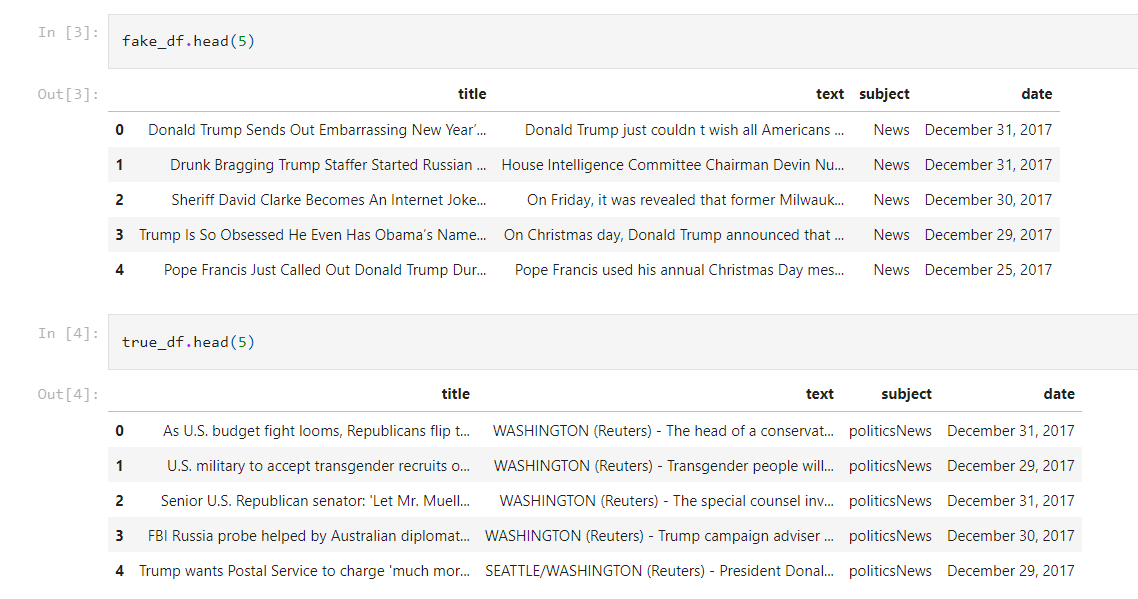
\includegraphics[width=0.8\linewidth]{img/quick-glance-at-data.PNG}
\end{figure}
\end{frame}

\begin{frame}{Preprocessing}
\begin{itemize}
\item Ta cần chỉnh sửa cấu trúc dataset:
\begin{itemize}
\item Loại bỏ các cột \texttt{title}, \texttt{subject} và \texttt{date}. Tạm thời ta không cần những cột này.
\item Thêm cột \texttt{class} để gán nhãn tin thật / tin giả.
\end{itemize}
\item Bước tiền xử lý:
\begin{itemize}
\item Loại bỏ dấu câu
\item Chuyển câu về dạng chữ thường
\item Loại bỏ số
\item Loại bỏ links, html tags và ký tự đặc biệt
\end{itemize}
\end{itemize}
\end{frame}

\begin{frame}{Preprocessing (cont.)}
\begin{columns}[c]
\column{.5\textwidth}
\begin{figure}
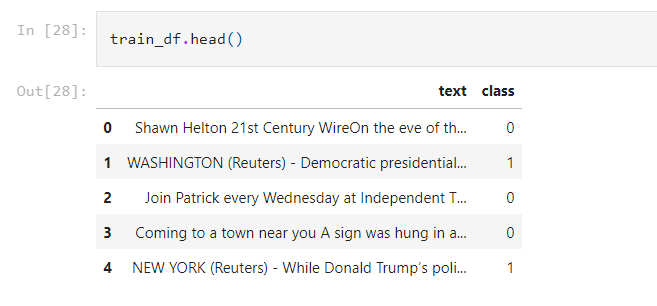
\includegraphics[width=0.98\linewidth]{img/train-csv.PNG}
\caption{Tập train, có gán nhãn}
\end{figure}

\column{.5\textwidth}
\begin{figure}
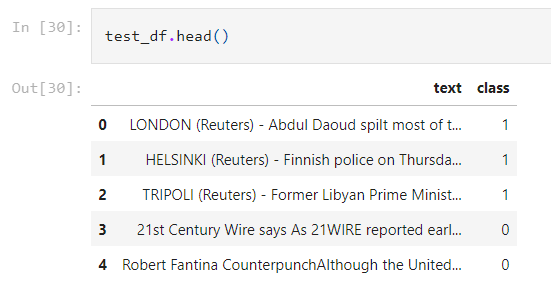
\includegraphics[width=0.9\linewidth]{img/test-csv.PNG}
\caption{Tập test, có gán nhãn}
\end{figure}
\end{columns}
\end{frame}

\begin{frame}{Preprocessing (cont.)}
\begin{columns}[c] % The "c" option specifies centered vertical alignment while the "t" option is used for top vertical alignment

\column{.4\textwidth} % Left column and width
\begin{block}{Trước}
LONDON (Reuters) - Abdul Daoud spilt most of the cappuccino into the saucer the first time he served Princess Diana, his nerves getting the better of him. Almost 20 years on since she was killed when her car crashed in a Paris tunnel, he still works surrounded by pictures of the woman he calls "the princess of the people" in his cafe, named Diana, his very personal attempt to keep her memory alive.
\end{block}
\pause
\column{.4\textwidth} % Right column and width
\begin{block}{Sau}
london  reuters    abdul daoud spilt most of the cappuccino into the saucer the first time he served princess diana  his nerves getting the better of him  almost  years on since she was killed when her car crashed in a paris tunnel  he still works surrounded by pictures of the woman he calls  the princess of the people  in his cafe  named diana  his very personal attempt to keep her memory alive 
\end{block}
\end{columns}
\end{frame}

\begin{frame}{Feature Extraction}
\begin{itemize}
\item Ta không `học thuộc` một câu, mà chỉ `học` những gì đặc trưng của câu đó.
\item Có nhiều cách trích xuất đặc trưng của câu: TF-IDF, BoW (đánh trọng số); GloVe, Word2Vec (chuyển câu thành dạng vector)
\item Một cách làm `tầm thường`: tính tần suất xuất hiện của những từ trong câu (trong đoạn văn / bài viết) và dựa trên tần suất lựa chọn các từ đặc trưng (TF).
\item Loại bỏ stopwords!
\end{itemize}
\end{frame}

\begin{frame}{Feature Extraction - TF-IDF}
\begin{itemize}
\item Term Frequency - Inverse Document Frequency
\item Phương pháp này làm giảm ảnh hưởng của những từ thường xuyên xuất hiện trong corpus.
\item Công thức biểu diễn trọng số $W$ của một từ (term) $t$ trong văn bản (document) $d$:
$$
W(d, t) = TF(d, t) \times \log\left(\frac{N}{df(t)}\right)
$$
Với $N$ là tổng số document, $df(t)$ là số lượng document chứa term $t$. $TF(d, t)$ là số lần xuất hiện của từ $t$ trong document $d$.
\end{itemize}
\end{frame}

\begin{frame}{Decision Tree (cây quyết định)}
Nhắc lại:
\begin{itemize}
\item Là phương pháp xuất hiện từ rất sớm và rất thành công trong nhiều lĩnh vực của text classification.
\item Ý tưởng: tạo một cấu trúc dữ liệu cây, mỗi nút là một thuộc tính của tập dữ liệu đã phân lớp.
\begin{itemize}
    \item Q: Làm sao biết thuộc tính nào là nút cha, thuộc tính nào là nút con?
    \item A: Feature Selection
\end{itemize}
\end{itemize}
\end{frame}

\begin{frame}{Decision Tree (cont.) - Feature Selection}
\begin{itemize}
\item Hàm số Entropy:
$$
H(\textbf{p}) = -\sum_{i = 1}^n p_i\log(p_i)
$$
Với $\textbf{p} = (p_1, p_2, .., p_n)$ là phân phối sao cho biến ngẫu nhiên $x$ nhận $n$ giá trị $(x_1, x_2, .., x_n)$ và xác suất lần lượt là $(p_1, p_2, .., p_n)$.

\begin{itemize}
\item Ví dụ: một tập dữ liệu có $p$ samples được gán nhãn \textit{positive} và $n$ samples được gán nhãn \textit{negative}. Khi đó entropy $H(\frac{p}{n + p}, \frac{n}{n + p})$ được tính như sau:
$$
H\left(\frac{p}{n + p}, \frac{n}{n + p}\right) = - \frac{p}{n + p}\log\left(\frac{p}{n + p}\right) - \frac{n}{n + p}\log\left(\frac{n}{n + p}\right)
$$
\end{itemize}
\end{itemize}
\end{frame}

\begin{frame}{Decision Tree (cont.) - Feature Selection}
\begin{itemize}
\item Chọn thuộc tính $A$ có $k$ giá trị khác nhau, chia tập train $E$ thành các tập con $\{E_1, E_2, .., E_k\}$. \textbf{Entropy kỳ vọng (EH)} còn lại sau khi chọn $A$ là một nút:
$$
EH(A) = \sum_{i = 1}^{k} \frac{p_i + n_i}{p + n} H\left(\frac{p_i}{n_i + p_i}, \frac{n_i}{n_i + p_i}\right)
$$
\item Độ đo \textbf{Information Gains}:
$$
A(I) = H\left(\frac{p}{n + p}, \frac{n}{n + p}\right) - EH(A)
$$
Ta sẽ chọn thuộc tính có Information Gain lớn nhất làm nút cha.
\end{itemize}
\end{frame}

\begin{frame}{Training \& testing}
\begin{figure}
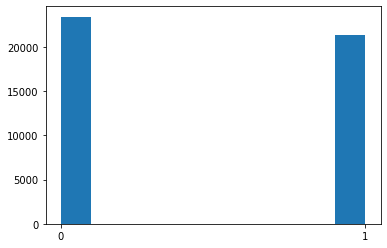
\includegraphics[width=0.35\linewidth]{img/real-fake-in-train.png}
\caption{Tương quan các lớp fake (0) và real (1) trong tập train}
\end{figure}

\begin{itemize}
\item Kích thước tập train 44798 samples, gồm các articles đã được gán nhãn 0 (fake) và 1 (real).
\item Kích thước tập test 100 samples = chọn ngẫu nhiên 50 article từ tập real + 50 article từ tập fake.
\item Sử dụng \texttt{sklearn.tree.DecisionTreeClassifier}
\end{itemize}
\end{frame}

\begin{frame}{Training \& testing (cont.)}
\begin{columns}[c]
\column{.35\textwidth}
\begin{figure}
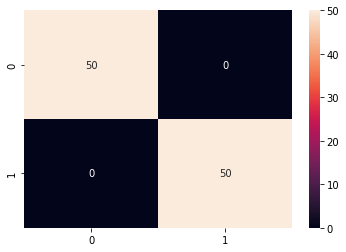
\includegraphics[width=0.8\linewidth]{img/train-result.png}
\caption{Heatmap kết quả testing}
\end{figure}
\column{.65\textwidth}
\begin{table}
\begin{tabular}{l l l l l}
\toprule
 & precision & recall & f1-score & support \\
\midrule
0 & 1.00 & 1.00 & 1.00 & 50 \\
1 & 1.00 & 1.00 & 1.00 & 50 \\
accuracy &   &   & 1.00 & 100 \\
macro avg & 1.00 & 1.00 & 1.00 & 100 \\
weighted avg & 1.00 & 1.00 & 1.00 & 100 \\
\bottomrule
\end{tabular}
\caption{\texttt{classification\_report} sau khi train}
\end{table}
\end{columns}

Nhận xét: độ chính xác gần như tuyệt đối (1.00)
\end{frame}

\section{Demo}
\begin{frame}{Demo}
    \Huge{\centerline{\textbf{Xem demo trực tiếp..}}}
\end{frame}

\begin{frame}{Tổng kết}
Ưu điểm:
\begin{itemize}
\item Decision Tree là thuật toán phân lớp phổ biến, dễ cài đặt.
\item Cho độ chính xác cao với tập dữ liệu nhỏ.
\item Thời gian huấn luyện nhanh.
\end{itemize}
Khuyết điểm:
\begin{itemize}
\item Dễ bị overfit. Xử lý: pruning
\item `Nhạy cảm` với sự xáo trộn dữ liệu.\cite{p1}
\end{itemize}
\end{frame}

\begin{frame}{QnA}
    \Huge{\centerline{\textbf{QnA}}}
\end{frame}

% \begin{frame}{Bullet Points}
%     \begin{itemize}
%         \item Lorem ipsum dolor sit amet, consectetur adipiscing elit
%         \item Aliquam blandit faucibus nisi, sit amet dapibus enim tempus eu
%         \item Nulla commodo, erat quis gravida posuere, elit lacus lobortis est, quis porttitor odio mauris at libero
%         \item Nam cursus est eget velit posuere pellentesque
%         \item Vestibulum faucibus velit a augue condimentum quis convallis nulla gravida
%     \end{itemize}
% \end{frame}

% %------------------------------------------------

% \begin{frame}{Blocks of Highlighted Text}
%     In this slide, some important text will be \alert{highlighted} because it's important. Please, don't abuse it.

%     \begin{block}{Block}
%         Sample text
%     \end{block}

%     \begin{alertblock}{Alertblock}
%         Sample text in red box
%     \end{alertblock}

%     \begin{examples}
%         Sample text in green box. The title of the block is ``Examples".
%     \end{examples}
% \end{frame}

% %------------------------------------------------

% \begin{frame}{Multiple Columns}
%     \begin{columns}[c] % The "c" option specifies centered vertical alignment while the "t" option is used for top vertical alignment

%         \column{.45\textwidth} % Left column and width
%         \textbf{Heading}
%         \begin{enumerate}
%             \item Statement
%             \item Explanation
%             \item Example
%         \end{enumerate}

%         \column{.5\textwidth} % Right column and width
%         Lorem ipsum dolor sit amet, consectetur adipiscing elit. Integer lectus nisl, ultricies in feugiat rutrum, porttitor sit amet augue. Aliquam ut tortor mauris. Sed volutpat ante purus, quis accumsan dolor.

%     \end{columns}
% \end{frame}

% %------------------------------------------------
% % \section{Second Section}
% %------------------------------------------------

% \begin{frame}{Table}
%     \begin{table}
%         \begin{tabular}{l l l}
%             \toprule
%             \textbf{Treatments} & \textbf{Response 1} & \textbf{Response 2} \\
%             \midrule
%             Treatment 1         & 0.0003262           & 0.562               \\
%             Treatment 2         & 0.0015681           & 0.910               \\
%             Treatment 3         & 0.0009271           & 0.296               \\
%             \bottomrule
%         \end{tabular}
%         \caption{Table caption}
%     \end{table}
% \end{frame}

% %------------------------------------------------

% \begin{frame}{Theorem}
%     \begin{theorem}[Mass--energy equivalence]
%         $E = mc^2$
%     \end{theorem}
% \end{frame}

% %------------------------------------------------

% \begin{frame}{Figure}
%     Uncomment the code on this slide to include your own image from the same directory as the template .TeX file.
%     % \begin{figure}
%     % \includegraphics[width=0.8\linewidth]{test}
%     % \end{figure}
% \end{frame}

% %------------------------------------------------

% \begin{frame}[fragile] % Need to use the fragile option when verbatim is used in the slide
%     \frametitle{Citation}
%     An example of the \verb|\cite| command to cite within the presentation:\\~

%     This statement requires citation \cite{p1}.
% \end{frame}

%------------------------------------------------
\section{Tài liệu}

\begin{frame}{Tài liệu}
    % Beamer does not support BibTeX so references must be inserted manually as below
    \footnotesize{
        \begin{thebibliography}{99}
            \bibitem[Kowsari, 2019]{p1} Kowsari and  Jafari Meimandi and  Heidarysafa and  Mendu and  Barnes and  Brown (2019)
            \newblock Text Classification Algorithms: A Survey
            \newblock \emph{Information} 10(4), 150
        \end{thebibliography}
    }
\end{frame}

%------------------------------------------------

\begin{frame}
    \Huge{\centerline{\textbf{Fin}}}
\end{frame}

%----------------------------------------------------------------------------------------

\end{document}